
\documentclass[11pt]{article}

\usepackage{amsmath}
\usepackage{graphicx}
\usepackage{booktabs}
\usepackage{geometry}
\geometry{margin=1in}

\title{The Prime Exponent Tree (PET): \\
A Structural View of Integer Factorization}

\author{Giancarlo Comneno}

\date{\today}

\begin{document}

\maketitle

\section{Introduction}

This paper explores the multiplicative structure of integers using a recursive
representation called the Prime Exponent Tree (PET). The goal is to study
structural patterns in integer factorizations independently of the actual
prime values.

\section{Prime Exponent Tree}

Given the prime factorization

\begin{equation}
N = \prod_i p_i^{e_i},
\end{equation}

each prime becomes a node and each exponent is recursively expanded
as another PET.

Example:

\begin{verbatim}
12 = 2^2 * 3

•
├─2
│  •
│  └─2
└─3
\end{verbatim}

\section{Dataset}

All integers from 2 to $10^6$ were processed to compute their PET structure.

Total integers analyzed:

\begin{center}
999,999
\end{center}

Only

\begin{center}
78 structural shapes
\end{center}

appear in this range.

\section{Height Distribution}

\begin{center}

\includegraphics[width=0.7\textwidth]{figures/height_distribution.png}
\end{center}

Most integers have very shallow PET trees.

\section{Branching Distribution}

\begin{center}

\includegraphics[width=0.7\textwidth]{figures/omega_distribution.png}
\end{center}

The peak occurs near $\omega(n)=3$, consistent with classical results
in analytic number theory.

\section{Entropy Growth}

\begin{center}
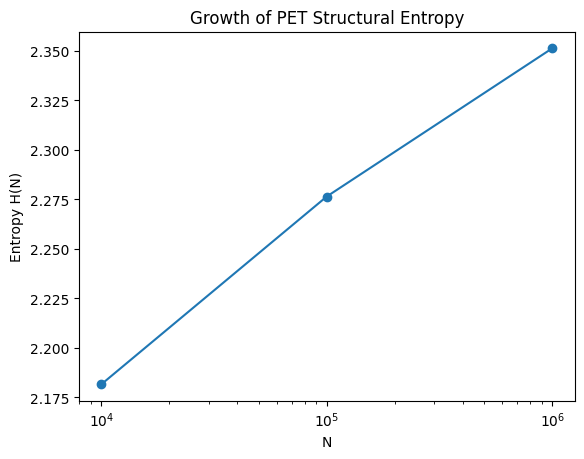
\includegraphics[width=0.7\textwidth]{figures/entropy_growth.png}
\end{center}

The entropy grows slowly with $N$ and appears roughly proportional
to $\log\log N$.

\section{Conclusion}

The PET representation reveals that the multiplicative structure
of integers occupies a very small combinatorial space. Despite the
vast number of integers, only a few structural shapes dominate.

\end{document}
